
% Eigener Beitrag: Beschreibung, Begründung, Aufzeigung, Methode, Fazit

\chapter{Anforderungsanalyse}
\label{sec:anforderungsanalyse}
Dieses Kapitel stellt die Stakeholders der Arbeit vor und zeigt deren Interaktionen mit dem Programm anhand der Anwendungsfälle auf. Schlussendlich werden daraus die funktionalen und nicht funktionalen Anforderungen abgeleitet.

\section{Stakeholders}
\label{sec:anforderungsanalyse:stakeholders}
In der \cref{fig:anfoderungsanalyse:stakeholders} sind die Stakeholders des Projekt abgebildet.
\begin{table}[h] 
	\caption{Stakeholders}
	\centering
	\rowcolors{1}{tablebodycolor}{tablerowcolor}
	\label{fig:anfoderungsanalyse:stakeholders}
	\begin{tabular}{ | c | L{5cm} | L{5cm} | } 
		\hline 
		\rowcolor{tableheadcolor}
		\bfseries Stakeholder & \bfseries Beschreibung & \bfseries Erwartungen \\ \hline 
		%Kunde & Besucher der Webseite, welcher Objekte buchen möchte und Werbung wahrnimmt. & Durch das Projekt sollen ihm passendere Objekte und Vorschläge angezeigt werden. \\ \hline 
		Interhome Marketing & Das Marketing ist für die Werbung auf der Interhome Webseite verantwortlich. & Möchte auf der Webseite passendere Angebote dem Benutzer darstellen.  \\ \hline 
		Interhome Einkauf & Abteilung, welche die Objekte einkauft, die auf der Interhome Webseite dargestellt werden. & Sie sollen durch das Projekt den Kunden besser verstehen und somit die Objekte einkaufen, welche von den Kunden gewünscht sind. \\ \hline 
		Interhome Tester & Testet das Programm und gibt Feedback, ob es korrekt arbeitet. & Eine gut entwickeltes Programm, welches bereits grundlegend von der Hotelplan Entwicklung getestet wurde. \\ \hline 
		Hotelplan Entwickler & Verantwortlich für die Umsetzung dieses Projektes. & Eine reibungslose Umsetzung des Projektes sowie eine konstruktive Kooperation mit den Testern. \\ \hline 
	\end{tabular}
\end{table} 

\section{Anwendungsfälle}
\label{sec:anforderungsanalyse:anwendungsfaelle}
In der \cref{fig:anfoderungsanalyse:anwendungsfaelle:1} werden die Anwendungsfälle des Programms dargestellt. Die Aktoren sind von der \cref{fig:anfoderungsanalyse:stakeholders} übernommen worden. 
\begin{figure}[H]
	\RawFloats
	\centering
	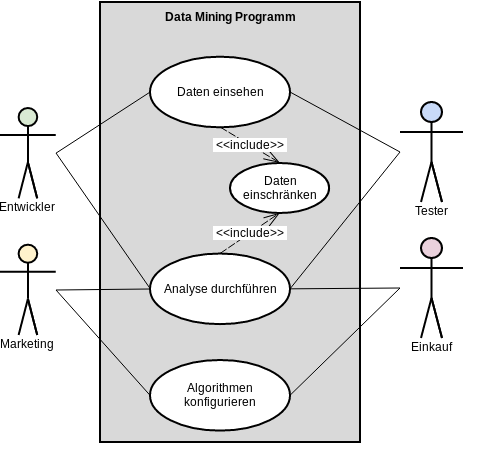
\includegraphics[width=0.7\textwidth]{images/usecase}
	\caption{Anwendungsfälle}
	\label{fig:anfoderungsanalyse:anwendungsfaelle:1}
\end{figure}

\paragraph{Daten einschränken} Es muss möglich sein die Daten einzuschränken. Dies sollte über vordefinierte Filterkriterien geschehen, die vom Benutzer ausgewählt werden können.

\paragraph{Daten einsehen} Um einen Überblick über die gesamten Daten zu haben, soll eine Ansicht erstellt werden, welche die Daten darstellt. Sie sollen zusätzlich gefiltert werden können, damit man die selbe Einschränkung vornehmen kann, welche auch bei den Algorithmen eingestellt werden kann.

\paragraph{Analyse durchführen} Es sollte möglich sein einen, oder mehrere Algorithmen auf die Daten anzuwenden und so eine Analyse durchzuführen. Die Daten sollen initial eingeschränkt werden können, um nur eine Untermenge zu analysieren.

\paragraph{Algorithmen konfigurieren} Der Benutzer soll die Möglichkeit besitzen die Algorithmen zu konfigurieren. Deshalb soll eine Ansicht erstellt werden, auf welcher vordefinierte Einstellungen angepasst werden können. Dies umfasst alle Parameter, die von den Algorithmen vorausgesetzt werden (siehe \cref{sec:recherche:algorithmen} \nameref{sec:recherche:algorithmen}) sowie das Gewicht zwischen numerischen und kategorischen Attributen der Distanzmessung (siehe \cref{sec:konzept:anwendungderalgorithmen:distanzmessung} \nameref{sec:konzept:anwendungderalgorithmen:distanzmessung}). Für die Beantwortung der Hypothesen aus dem \cref{sec:einleitung:ziel:hypothesen} \nameref{sec:einleitung:ziel:hypothesen} müssen die von den Algorithmen zu analysieren Attribute eingeschränkt werden können. Zum Beispiel benötigt Hypothese 1 nur das Land des Kunden. Deshalb soll es eine Konfiguration geben, mit welchem die Algorithmen so angepasst werden, dass nur dieses Attribut (Land des Kunden) beachtet wird.



\section{Ablauf}
\label{sec:anforderungsanalyse:ablauf}
%In diesem Abschnitt wird der Ablauf von der Dateneinschränkung bis zum anbringen von Änderungswünschen erklärt.
%
%Zuerst kann der Benutzer die Daten einschränken. Der gesamte oder gefilterte Datenbestand wird anschliessend von einem Algorithmus analysiert. Daraufhin kann der Benutzer die Resultate überprüfen und wenn Fehler aufgedeckt werden diese an den Entwickler weiterleiten.
%Visualisiert wird der Ablauf in \cref{fig:anfoderungsanalyse:ablauf:1}.
In \cref{fig:anfoderungsanalyse:ablauf:1} sind die Abläufe der Anwendungsfälle in einem Flowchart visualisiert. 

Der Hauptfall ist "`Analyse durchführen"', welcher als Erstes "`Daten laden"' aufruft. Dort werden alle Einträge in der Datenbasis geladen, anschliessend, wenn vom Benutzer gewünscht, gefiltert und schlussendlich zurückgegeben. Wenn das "`Daten laden"' beendet ist, wird die Konfigurationen geladen und der Algorithmus angewendet.

Der Anwendungsfall "`Daten einsehen"' lädt die Daten auf die selbe Weise wie "`Analyse durchführen"'. Anschliessend werden die Daten ausgegeben, sodass der Benutzer sie einsehen kann.

Der letzte Anwendungsfall ist die Konfiguration der Algorithmen. Dazu werden die einstellbaren Werte dem Benutzer ausgegeben, damit er diese ändern kann. Die Änderungen werden anschliessend in eine Konfigurationsdatei geschrieben, damit sie bei der nächsten Analyse verwendet werden können.

\begin{figure}[H]
	\RawFloats
	\centering
	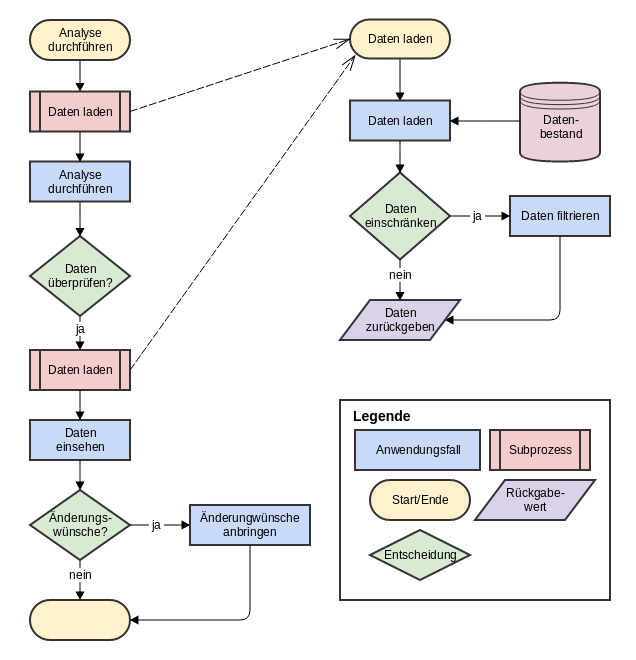
\includegraphics[width=0.9\textwidth]{images/flowchart}
	\caption{Ablauf}
	\label{fig:anfoderungsanalyse:ablauf:1}
\end{figure}

\section{Funktionale Anforderungen}
\label{sec:anforderungsanalyse:funktionaleanforderung}
Nachfolgend werden die funktionale Anforderungen an das Programm aufgeführt. Abgeleitet wurden diese aus den Anwendungsfällen, dem Ablauf und den Hypothesen.

%\todo{FA1: Welche Felder? Aus Hypothese}
\begin{table}[H] 
	\caption{FA1: Häufigkeitsanalyse der Attribute}
	\centering
	\rowcolors{1}{tablebodycolor}{tablerowcolor}
	\label{fig:anforderungsanalyse:funktionaleanforderung:fa1}
	\begin{tabular}{ | l | L{10cm} | } 
		\hline 
		\rowcolor{tableheadcolor}
		\multicolumn{2}{|l|}{\bfseries ID: FA1} \\ \hline 
		Titel & Häufigkeitsanalyse der Attribute \\ \hline 
		Beschreibung & Das Programm muss für die Gewinnung neues Wissens aus den bisherigen Buchungen von Interhome gestaltet werden. Dazu sollen Algorithmen eingesetzt werden, die folgende beispielhaften Fragestellungen beantworten können:
		\begin{enumerate}
		\item Welche Attribute werden von Schweizern im Winter gebucht?
		\item Welche Destination wird von Kunden im Tessin am meisten gebucht?
		\end{enumerate}
		
		Als Antwort sollte der Algorithmus eine Liste von Attributen zurückliefern. Auf die obigen Beispiele könnte dies folgende sein: 
		\begin{enumerate}
		\item Objekte in Süditalien mit einem Pool.
		\item Objekte in Zermatt und mindestens 3 Schlafzimmern.
		\end{enumerate} \\ \hline 
		Abhängigkeit & \\ \hline 
	\end{tabular}
\end{table}

\begin{table}[H] 
	\caption{FA2: Nachvollziehbarkeit der Attributanalyse}
	\centering
	\rowcolors{1}{tablebodycolor}{tablerowcolor}
	\label{fig:anforderungsanalyse:funktionaleanforderung:fa2}
	\begin{tabular}{ | l | L{10cm} | } 
		\hline 
		\rowcolor{tableheadcolor}
		\multicolumn{2}{|l|}{\bfseries ID: FA2} \\ \hline 
		Titel & Nachvollziehbarkeit der Attributanalyse \\ \hline 
		Beschreibung & Die Resultate aus FA1 sollten nachvollziehbar sein. Es sollte dem Benutzer verständlich gemacht werden, wieso der Algorithmus diese Attribute gewählt hat. Jede Eigenschaft sollte demnach mit einer Anzahl oder einer Prozentzahl versehen sein. Zum Beispiel:
			\begin{enumerate}
			\item Sütitalien (223 von 319) und Pool (150 von 319)
			\item Luxushäuser (53\%), Grill (35\%) und 3 Zimmer (32\%)
			\end{enumerate} \\ \hline 
		Abhängigkeit & FA1 \\ \hline 
	\end{tabular}
\end{table}

\begin{table}[H] 
	\caption{FA3: Häufigkeitsanalyse auf einer Untermenge der Daten}
	\centering
	\rowcolors{1}{tablebodycolor}{tablerowcolor}
	\label{fig:anforderungsanalyse:funktionaleanforderung:fa3}
	\begin{tabular}{ | l | L{10cm} | } 
		\hline 
		\rowcolor{tableheadcolor}
		\multicolumn{2}{|l|}{\bfseries ID: FA3} \\ \hline 
		Titel & Häufigkeitsanalyse auf einer Untermenge der Daten \\ \hline 
		Beschreibung & Eine Häufigkeitsanalyse solle gemäss FA1 auch auf einer Untermenge der Daten möglich sein. Der Benutzer soll befähigt werden den Datenbestand vor der Analyse einzuschränken. \\ \hline 
		Abhängigkeit & FA1 \\ \hline 
	\end{tabular}
\end{table}

\begin{table}[H] 
	\caption{FA4: Stammdaten einsehen}
	\centering
	\rowcolors{1}{tablebodycolor}{tablerowcolor}
	\label{fig:anforderungsanalyse:funktionaleanforderung:fa4}
	\begin{tabular}{ | l | L{10cm} | } 
		\hline 
		\rowcolor{tableheadcolor}
		\multicolumn{2}{|l|}{\bfseries ID: FA4} \\ \hline 
		Titel & Stammdaten einsehen \\ \hline 
		Beschreibung & Um die Analyse der Daten zu validieren, sollte es möglich sein die Stammdaten einzusehen. Deshalb sollen im Programm alle Daten dargestellt und vom Benutzer durchstöbert werden können. \\ \hline 
		Abhängigkeit & \\ \hline 
	\end{tabular}
\end{table}

\begin{table}[H] 
	\caption{FA5: Untermenge der Stammdaten einsehen}
	\centering
	\rowcolors{1}{tablebodycolor}{tablerowcolor}
	\label{fig:anforderungsanalyse:funktionaleanforderung:fa5}
	\begin{tabular}{ | l | L{10cm} | } 
		\hline 
		\rowcolor{tableheadcolor}
		\multicolumn{2}{|l|}{\bfseries ID: FA5} \\ \hline 
		Titel & Untermenge der Stammdaten einsehen \\ \hline 
		Beschreibung & Eine Untermenge der Stammdaten soll gemäss FA3 eingesehen werden können. Diese sollen gleich wie in FA2 einschränkbar sein. \\ \hline 
		Abhängigkeit & FA1 \& FA4 \\ \hline 
	\end{tabular}
\end{table}

\begin{table}[H] 
	\caption{FA6: Mixed data types}
	\centering
	\rowcolors{1}{tablebodycolor}{tablerowcolor}
	\label{fig:anforderungsanalyse:funktionaleanforderung:fa6}
	\begin{tabular}{ | l | L{10cm} | } 
		\hline 
		\rowcolor{tableheadcolor}
		\multicolumn{2}{|l|}{\bfseries ID: FA6} \\ \hline 
		Titel & Mixed data types \\ \hline 
		Beschreibung & Da die Buchungen von Interhome numerische (z.B. Anzahl Personen, Geolocations) und kategorische Daten (z.B. Aircondition vorhanden?, Objekttyp) beinhalten, müssen die Algorithmen in der Lage sein mit beiden Datentypen umgehen zu können. \\ \hline 
		Abhängigkeit & \\ \hline 
	\end{tabular}
\end{table}

\begin{table}[H] 
	\caption{FA7: Algorithmen konfigurieren}
	\centering
	\rowcolors{1}{tablebodycolor}{tablerowcolor}
	\label{fig:anforderungsanalyse:funktionaleanforderung:fa8}
	\begin{tabular}{ | l | L{10cm} | } 
		\hline 
		\rowcolor{tableheadcolor}
		\multicolumn{2}{|l|}{\bfseries ID: FA7} \\ \hline 
		Titel & Algorithmen konfigurieren \\ \hline 
		Beschreibung & Der Benutzer soll die Möglichkeit besitzen folgende Konfigurationen am Programm vorzunehmen:
		\begin{itemize}
			\item Apriori:
			\begin{itemize}
				\item Mindestsupport $minsup$
			\end{itemize}
			\item k-prototype:
			\begin{itemize}
				\item Anzahl Clusters $k$
			\end{itemize}
			\item DBScan:
			\begin{itemize}
				\item Radius $\epsilon$
				\item Minimum Anzahl an Instanzen $minpts$
			\end{itemize}
			\item Gewicht zwischen numerischen und kategorischen Attributen $\gamma$ in der Distanzberechnung (siehe \cref{sec:konzept:anwendungderalgorithmen:distanzmessung} \nameref{sec:konzept:anwendungderalgorithmen:distanzmessung}).
			\item Zu verwendende Attribute der Algorithmen.
		\end{itemize}
		 \\ \hline 
		Abhängigkeit & \\ \hline 
	\end{tabular}
\end{table}


\section{Nicht funktionale Anforderungen}
\label{sec:anforderungsanalyse:nichtfunktionaleanforderung}
Nachfolgend sind die nicht funktionalen Anforderungen an das Programm spezifiziert. Diese gehen nicht auf die Funktionalität der Applikation ein, sondern auf die Komplexität, Performanz, etc.

%\begin{table}[H] 
%	\caption{NFA1: Geschwindigkeit}
%	\centering
%	\rowcolors{1}{tablebodycolor}{tablerowcolor}
%	\label{fig:anforderungsanalyse:nichtfunktionaleanforderung:nfa1}
%	\begin{tabular}{ | l | L{10cm} | } 
%		\hline 
%		\rowcolor{tableheadcolor}
%		\multicolumn{2}{|l|}{\bfseries ID: NFA1} \\ \hline 
%		Titel & Geschwindigkeit \\ \hline 
%		Beschreibung & Da das Programm explorativ verwendet werden soll, muss das Programm eine zügige Antwortszeit aufweisen. Deshalb soll die Attributanalyse innerhalb von 30 Sekunden Resultate liefern können. Die Algorithmen sollten daher maximal ein super-lineares Wachstum ($\mathcal{O}(n\,log\,n)$) aufweisen. \\ \hline 
%		Abhängigkeit & \\ \hline 
%		Status & Offen \\ \hline 
%	\end{tabular}
%\end{table}
%\todo{apriori O(n log n)?}

\begin{table}[H] 
	\caption{NFA1: Komplexität}
	\centering
	\rowcolors{1}{tablebodycolor}{tablerowcolor}
	\label{fig:anforderungsanalyse:nichtfunktionaleanforderung:nfa1}
	\begin{tabular}{ | l | L{10cm} | } 
		\hline 
		\rowcolor{tableheadcolor}
		\multicolumn{2}{|l|}{\bfseries ID: NFA1} \\ \hline 
		Titel & Komplexität \\ \hline 
		Beschreibung & Verwendet wird das Programm von Interhome Mitarbeitern ohne Vorwissen im Data Mining. Deshalb sollte die Bedingung möglichst einfach ausgelegt sein. \\ \hline 
		Abhängigkeit & \\ \hline 
	\end{tabular}
\end{table}

\begin{table}[H] 
	\caption{NFA2: Modularität}
	\centering
	\rowcolors{1}{tablebodycolor}{tablerowcolor}
	\label{fig:anforderungsanalyse:nichtfunktionaleanforderung:nfa2}
	\begin{tabular}{ | l | L{10cm} | } 
		\hline 
		\rowcolor{tableheadcolor}
		\multicolumn{2}{|l|}{\bfseries ID: NFA2} \\ \hline 
		Titel & Modularität \\ \hline 
		Beschreibung & In Zukunft ist zu erwarten, dass das Programm um weitere Techniken des Data Mining und weitere Attribute in der Datenbasis erweitert werden kann. Deshalb sollte es modular aufgebaut werden, damit weitere Algorithmen und Attribute leicht hinzugefügt werden können. Zusätzlich sollte durch die Modularität die Verständlichkeit des Programms erhöht werden, so dass zukünftige Entwickler sich besser in die Umsetzung einarbeiten können. \\ \hline 
		Abhängigkeit & \\ \hline 
	\end{tabular}
\end{table}

\begin{table}[H] 
	\caption{NFA3: Erweiterbarkeit der Daten}
	\centering
	\rowcolors{1}{tablebodycolor}{tablerowcolor}
	\label{fig:anforderungsanalyse:nichtfunktionaleanforderung:nfa3}
	\begin{tabular}{ | l | L{10cm} | } 
		\hline 
		\rowcolor{tableheadcolor}
		\multicolumn{2}{|l|}{\bfseries ID: NFA3} \\ \hline 
		Titel & Erweiterbarkeit der Daten \\ \hline 
		Beschreibung & Um die Aktualität der Informationen zu gewährleisten, soll der Datenbestand in Zukunft leicht erweitert werden können. \\ \hline 
		Abhängigkeit & \\ \hline 
	\end{tabular}
\end{table}
 
 \begin{table}[H] 
	\caption{NFA4: Kosten}
	\centering
	\rowcolors{1}{tablebodycolor}{tablerowcolor}
	\label{fig:anforderungsanalyse:nichtfunktionaleanforderung:nfa4}
	\begin{tabular}{ | l | L{10cm} | } 
		\hline 
		\rowcolor{tableheadcolor}
		\multicolumn{2}{|l|}{\bfseries ID: NFA4} \\ \hline 
		Titel & Kosten \\ \hline 
		Beschreibung & Falls ein bestehendes Programm eingesetzt wird, sollen folgende Kostenfaktoren beachtet werden: 
		\begin{itemize}
		\item Die Applikation sollte kostenlos einsetzbar sein. Sie benötigt demnach eine der folgenden Lizenzmodelle:
		\begin{itemize}
		\item OpenSource. Software kann verwendet und angepasst werden (siehe \url{https://opensource.org/licenses}).
		\item Freeware. Software kann verwendet, jedoch nicht angepasst werden.
		\item Studenten Lizenz. Software kann als Student kostenlos eingesetzt werden.
		\end{itemize}
		\item Die Entwicklung wird privat auf einem Linux Rechner durchgeführt und zeitweise auch bei der Arbeit auf Windows Computern, die von Hotelplan Management AG bereitgestellt werden.
		Demnach ist es nötig, dass die Software unter Linux sowie auch Windows gestartet werden kann.
		\item Da der Datenbestand 133'001 Einträge umfasst, muss die Plattform und das Lizenzmodell diese Anzahl an Items unterstützen.
		\end{itemize}\\ \hline 
		Abhängigkeit & \\ \hline 
	\end{tabular}
\end{table}

